\documentclass[]{article}
\usepackage{lmodern}
\usepackage{amssymb,amsmath}
\usepackage{ifxetex,ifluatex}
\usepackage{fixltx2e} % provides \textsubscript
\ifnum 0\ifxetex 1\fi\ifluatex 1\fi=0 % if pdftex
  \usepackage[T1]{fontenc}
  \usepackage[utf8]{inputenc}
\else % if luatex or xelatex
  \ifxetex
    \usepackage{mathspec}
    \usepackage{xltxtra,xunicode}
  \else
    \usepackage{fontspec}
  \fi
  \defaultfontfeatures{Mapping=tex-text,Scale=MatchLowercase}
  \newcommand{\euro}{€}
\fi
% use upquote if available, for straight quotes in verbatim environments
\IfFileExists{upquote.sty}{\usepackage{upquote}}{}
% use microtype if available
\IfFileExists{microtype.sty}{%
\usepackage{microtype}
\UseMicrotypeSet[protrusion]{basicmath} % disable protrusion for tt fonts
}{}
\usepackage[margin=1in]{geometry}
\usepackage{color}
\usepackage{fancyvrb}
\newcommand{\VerbBar}{|}
\newcommand{\VERB}{\Verb[commandchars=\\\{\}]}
\DefineVerbatimEnvironment{Highlighting}{Verbatim}{commandchars=\\\{\}}
% Add ',fontsize=\small' for more characters per line
\usepackage{framed}
\definecolor{shadecolor}{RGB}{248,248,248}
\newenvironment{Shaded}{\begin{snugshade}}{\end{snugshade}}
\newcommand{\KeywordTok}[1]{\textcolor[rgb]{0.13,0.29,0.53}{\textbf{{#1}}}}
\newcommand{\DataTypeTok}[1]{\textcolor[rgb]{0.13,0.29,0.53}{{#1}}}
\newcommand{\DecValTok}[1]{\textcolor[rgb]{0.00,0.00,0.81}{{#1}}}
\newcommand{\BaseNTok}[1]{\textcolor[rgb]{0.00,0.00,0.81}{{#1}}}
\newcommand{\FloatTok}[1]{\textcolor[rgb]{0.00,0.00,0.81}{{#1}}}
\newcommand{\CharTok}[1]{\textcolor[rgb]{0.31,0.60,0.02}{{#1}}}
\newcommand{\StringTok}[1]{\textcolor[rgb]{0.31,0.60,0.02}{{#1}}}
\newcommand{\CommentTok}[1]{\textcolor[rgb]{0.56,0.35,0.01}{\textit{{#1}}}}
\newcommand{\OtherTok}[1]{\textcolor[rgb]{0.56,0.35,0.01}{{#1}}}
\newcommand{\AlertTok}[1]{\textcolor[rgb]{0.94,0.16,0.16}{{#1}}}
\newcommand{\FunctionTok}[1]{\textcolor[rgb]{0.00,0.00,0.00}{{#1}}}
\newcommand{\RegionMarkerTok}[1]{{#1}}
\newcommand{\ErrorTok}[1]{\textbf{{#1}}}
\newcommand{\NormalTok}[1]{{#1}}
\usepackage{graphicx}
\makeatletter
\def\maxwidth{\ifdim\Gin@nat@width>\linewidth\linewidth\else\Gin@nat@width\fi}
\def\maxheight{\ifdim\Gin@nat@height>\textheight\textheight\else\Gin@nat@height\fi}
\makeatother
% Scale images if necessary, so that they will not overflow the page
% margins by default, and it is still possible to overwrite the defaults
% using explicit options in \includegraphics[width, height, ...]{}
\setkeys{Gin}{width=\maxwidth,height=\maxheight,keepaspectratio}
\ifxetex
  \usepackage[setpagesize=false, % page size defined by xetex
              unicode=false, % unicode breaks when used with xetex
              xetex]{hyperref}
\else
  \usepackage[unicode=true]{hyperref}
\fi
\hypersetup{breaklinks=true,
            bookmarks=true,
            pdfauthor={Fernando Martínez Plumed},
            pdftitle={Reproducible Research: Peer Assessment 1},
            colorlinks=true,
            citecolor=blue,
            urlcolor=blue,
            linkcolor=magenta,
            pdfborder={0 0 0}}
\urlstyle{same}  % don't use monospace font for urls
\setlength{\parindent}{0pt}
\setlength{\parskip}{6pt plus 2pt minus 1pt}
\setlength{\emergencystretch}{3em}  % prevent overfull lines
\setcounter{secnumdepth}{0}

%%% Use protect on footnotes to avoid problems with footnotes in titles
\let\rmarkdownfootnote\footnote%
\def\footnote{\protect\rmarkdownfootnote}

%%% Change title format to be more compact
\usepackage{titling}

% Create subtitle command for use in maketitle
\newcommand{\subtitle}[1]{
  \posttitle{
    \begin{center}\large#1\end{center}
    }
}

\setlength{\droptitle}{-2em}
  \title{Reproducible Research: Peer Assessment 1}
  \pretitle{\vspace{\droptitle}\centering\huge}
  \posttitle{\par}
  \author{Fernando Martínez Plumed}
  \preauthor{\centering\large\emph}
  \postauthor{\par}
  \predate{\centering\large\emph}
  \postdate{\par}
  \date{23th of September,2015}



\begin{document}

\maketitle


\section{Loading and preprocessing the
data}\label{loading-and-preprocessing-the-data}

Load libraries

\begin{Shaded}
\begin{Highlighting}[]
 \CommentTok{# List of packages for session}
\NormalTok{.packages <-}\StringTok{ }\KeywordTok{c}\NormalTok{(}\StringTok{"dplyr"}\NormalTok{,}\StringTok{"reshape2"}\NormalTok{,}\StringTok{"lubridate"}\NormalTok{,}\StringTok{"ggplot2"}\NormalTok{, }\StringTok{"xtable"}\NormalTok{)}

\NormalTok{installed <-}\StringTok{ }\NormalTok{function(pack)\{pack %in%}\StringTok{ }\KeywordTok{installed.packages}\NormalTok{()[,}\DecValTok{1}\NormalTok{]\}}

\NormalTok{load.pack <-}\StringTok{ }\NormalTok{function(packs)\{}
  \NormalTok{for (p in packs)\{}
    \NormalTok{if (!}\KeywordTok{installed}\NormalTok{(p))\{}
      \KeywordTok{install.packages}\NormalTok{(p)}
    \NormalTok{\}}
    \KeywordTok{require}\NormalTok{(p, }\DataTypeTok{character.only=}\OtherTok{TRUE}\NormalTok{)}
    
  \NormalTok{\}}
\NormalTok{\}}

\KeywordTok{load.pack}\NormalTok{(.packages)}
\end{Highlighting}
\end{Shaded}

Load the data (i.e.~read.csv())

\begin{Shaded}
\begin{Highlighting}[]
\NormalTok{Activity <-}\StringTok{ }\KeywordTok{tbl_df}\NormalTok{(}\KeywordTok{read.csv}\NormalTok{(}\StringTok{"activity.csv"}\NormalTok{))}
\NormalTok{Activity}
\end{Highlighting}
\end{Shaded}

\begin{verbatim}
## Source: local data frame [17,568 x 3]
## 
##    steps       date interval
## 1     NA 2012-10-01        0
## 2     NA 2012-10-01        5
## 3     NA 2012-10-01       10
## 4     NA 2012-10-01       15
## 5     NA 2012-10-01       20
## 6     NA 2012-10-01       25
## 7     NA 2012-10-01       30
## 8     NA 2012-10-01       35
## 9     NA 2012-10-01       40
## 10    NA 2012-10-01       45
## ..   ...        ...      ...
\end{verbatim}

Process/transform the data (if necessary) into a format suitable for
your analysis: Date from factor to Date

\begin{Shaded}
\begin{Highlighting}[]
\NormalTok{Activity$date <-}\StringTok{ }\KeywordTok{ymd}\NormalTok{(Activity$date)}
\CommentTok{#Activity <- Activity[complete.cases(Activity)]}
\end{Highlighting}
\end{Shaded}

\section{What is mean total number of steps taken per
day?}\label{what-is-mean-total-number-of-steps-taken-per-day}

For this part of the assignment, you can ignore the missing values in
the dataset.

Make a histogram of the total number of steps taken each day

\begin{Shaded}
\begin{Highlighting}[]
\NormalTok{Activity.day <-}\StringTok{ }\KeywordTok{group_by}\NormalTok{(Activity, date) }
\NormalTok{Activity.day}
\end{Highlighting}
\end{Shaded}

\begin{verbatim}
## Source: local data frame [17,568 x 3]
## Groups: date
## 
##    steps       date interval
## 1     NA 2012-10-01        0
## 2     NA 2012-10-01        5
## 3     NA 2012-10-01       10
## 4     NA 2012-10-01       15
## 5     NA 2012-10-01       20
## 6     NA 2012-10-01       25
## 7     NA 2012-10-01       30
## 8     NA 2012-10-01       35
## 9     NA 2012-10-01       40
## 10    NA 2012-10-01       45
## ..   ...        ...      ...
\end{verbatim}

\begin{Shaded}
\begin{Highlighting}[]
\NormalTok{Activity.day.sum <-}\StringTok{ }\KeywordTok{summarise}\NormalTok{(Activity.day, }\DataTypeTok{total=} \KeywordTok{sum}\NormalTok{(steps,}\DataTypeTok{na.rm =} \NormalTok{T))}



\NormalTok{g <-}\StringTok{ }\KeywordTok{ggplot}\NormalTok{(}\KeywordTok{select}\NormalTok{(Activity.day.sum, date, total), }\KeywordTok{aes}\NormalTok{(}\DataTypeTok{x=}\NormalTok{total))}
\NormalTok{g +}\StringTok{ }\KeywordTok{geom_histogram}\NormalTok{(}\DataTypeTok{binwidth=}\DecValTok{5000}\NormalTok{) +}\StringTok{ }\KeywordTok{ggtitle}\NormalTok{(}\StringTok{"Histogram of total number of steps per day"}\NormalTok{)+}\StringTok{ }\KeywordTok{xlab}\NormalTok{(}\StringTok{"Total steps per day"}\NormalTok{)}
\end{Highlighting}
\end{Shaded}

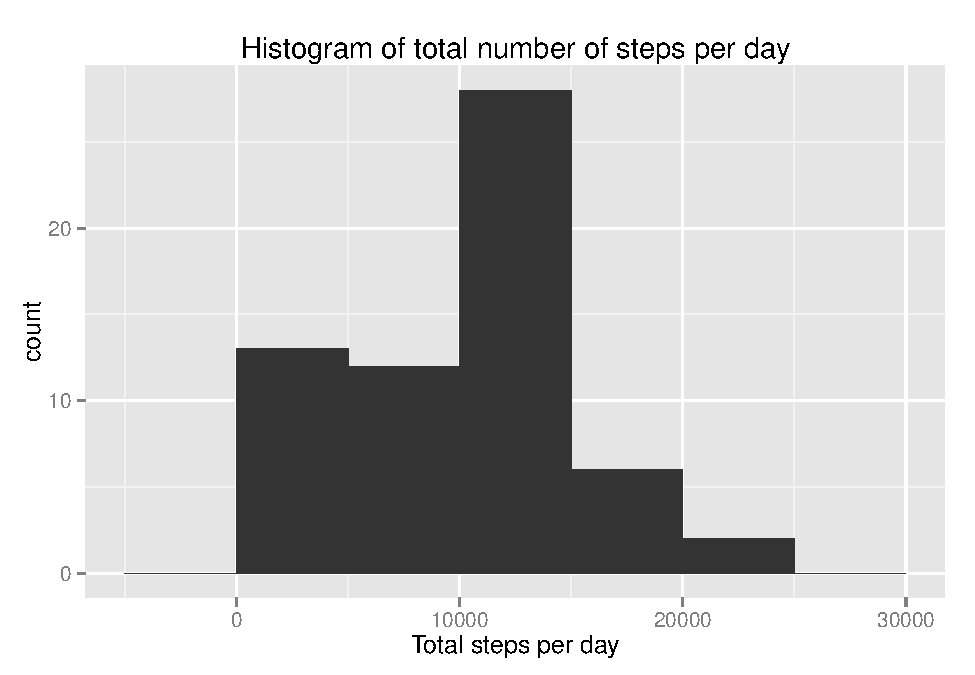
\includegraphics{PA1_template_files/figure-latex/unnamed-chunk-4-1.pdf}

\begin{Shaded}
\begin{Highlighting}[]
\NormalTok{mean <-}\StringTok{ }\KeywordTok{trunc}\NormalTok{(}\KeywordTok{mean}\NormalTok{(Activity.day.sum$total, }\DataTypeTok{na.rm =} \NormalTok{T))}
\NormalTok{median <-}\StringTok{ }\KeywordTok{trunc}\NormalTok{(}\KeywordTok{median}\NormalTok{(Activity.day.sum$total, }\DataTypeTok{na.rm =} \NormalTok{T))}
\end{Highlighting}
\end{Shaded}

\section{What is the average daily activity
pattern?}\label{what-is-the-average-daily-activity-pattern}

Make a time series plot (i.e.~type = ``l'') of the 5-minute interval
(x-axis) and the average number of steps taken, averaged across all days
(y-axis)

\begin{Shaded}
\begin{Highlighting}[]
\NormalTok{Activity.interval <-}\StringTok{ }\KeywordTok{group_by}\NormalTok{(Activity, interval) }
\NormalTok{Activity.interval.avg <-}\StringTok{ }\KeywordTok{summarise}\NormalTok{(Activity.interval, }\DataTypeTok{avg =} \KeywordTok{mean}\NormalTok{(steps, }\DataTypeTok{na.rm=}\NormalTok{T))}
  

\NormalTok{g <-}\StringTok{ }\KeywordTok{ggplot}\NormalTok{(Activity.interval.avg, }\KeywordTok{aes}\NormalTok{(interval, avg))}
\NormalTok{g +}\StringTok{ }\KeywordTok{geom_line}\NormalTok{() +}\StringTok{ }\KeywordTok{ggtitle}\NormalTok{(}\StringTok{"Average number of steps over all days"}\NormalTok{) +}\StringTok{ }\KeywordTok{xlab}\NormalTok{(}\StringTok{"Interval"}\NormalTok{) +}\StringTok{ }\KeywordTok{ylab}\NormalTok{(}\StringTok{"Average number of steps"}\NormalTok{)}
\end{Highlighting}
\end{Shaded}

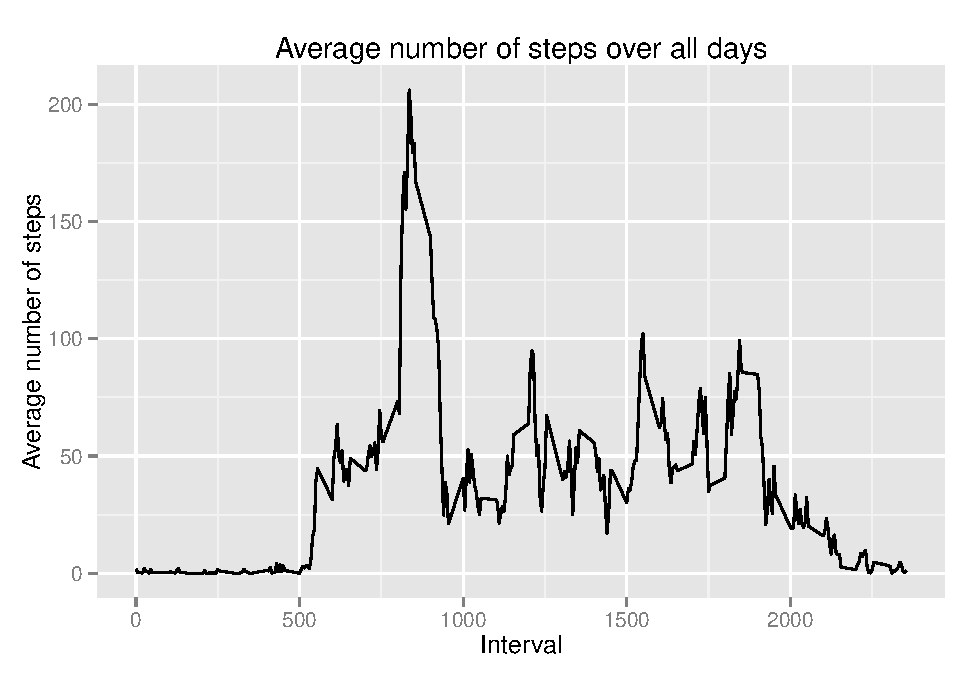
\includegraphics{PA1_template_files/figure-latex/unnamed-chunk-6-1.pdf}

\begin{Shaded}
\begin{Highlighting}[]
\NormalTok{max <-}\StringTok{ }\NormalTok{Activity.interval.avg[}\KeywordTok{which.max}\NormalTok{(Activity.interval.avg$avg),]$interval}
\end{Highlighting}
\end{Shaded}

Which 5-minute interval, on average across all the days in the dataset,
contains the maximum number of steps? 835

\section{Imputing missing values}\label{imputing-missing-values}

Note that there are a number of days/intervals where there are missing
values (coded as NA). The presence of missing days may introduce bias
into some calculations or summaries of the data.

\begin{Shaded}
\begin{Highlighting}[]
\NormalTok{rowsNA <-}\StringTok{ }\KeywordTok{sum}\NormalTok{(}\KeywordTok{is.na}\NormalTok{(Activity))}
\end{Highlighting}
\end{Shaded}

The total number of missing values in the dataset (i.e.~the total number
of rows with NAs) : 2304

Replacing NA's with the mean for that 5-minute interval. Creating a new
dataset that is equal to the original dataset but with the missing data
filled in.

\begin{Shaded}
\begin{Highlighting}[]
\NormalTok{Activity.clean <-}\StringTok{ }\NormalTok{Activity}
\NormalTok{for(i in }\DecValTok{1}\NormalTok{:}\KeywordTok{nrow}\NormalTok{(Activity.clean))\{}
  \NormalTok{if (}\KeywordTok{is.na}\NormalTok{(Activity.clean$steps[i]))\{}
    \NormalTok{thisInterval <-}\StringTok{ }\NormalTok{Activity.clean$interval[i]}
    \NormalTok{AvgValue <-}\StringTok{ }\NormalTok{Activity.interval.avg[Activity.interval.avg$interval ==}\StringTok{ }\NormalTok{thisInterval,]$avg}
    \NormalTok{Activity.clean$steps[i]<-}\StringTok{ }\NormalTok{AvgValue}
  \NormalTok{\}}
\NormalTok{\}}
\end{Highlighting}
\end{Shaded}

Histogram of the total number of steps taken each day and the mean and
median total number of steps taken per day. Do these values differ from
the estimates from the first part of the assignment? What is the impact
of imputing missing data on the estimates of the total daily number of
steps?

\begin{Shaded}
\begin{Highlighting}[]
\NormalTok{Activity.clean.day <-}\StringTok{ }\KeywordTok{group_by}\NormalTok{(Activity.clean, date) }
\NormalTok{Activity.clean.day}
\end{Highlighting}
\end{Shaded}

\begin{verbatim}
## Source: local data frame [17,568 x 3]
## Groups: date
## 
##        steps       date interval
## 1  1.7169811 2012-10-01        0
## 2  0.3396226 2012-10-01        5
## 3  0.1320755 2012-10-01       10
## 4  0.1509434 2012-10-01       15
## 5  0.0754717 2012-10-01       20
## 6  2.0943396 2012-10-01       25
## 7  0.5283019 2012-10-01       30
## 8  0.8679245 2012-10-01       35
## 9  0.0000000 2012-10-01       40
## 10 1.4716981 2012-10-01       45
## ..       ...        ...      ...
\end{verbatim}

\begin{Shaded}
\begin{Highlighting}[]
\NormalTok{Activity.clean.day.sum <-}\StringTok{ }\KeywordTok{summarise}\NormalTok{(Activity.clean.day, }\DataTypeTok{total=} \KeywordTok{sum}\NormalTok{(steps))}


\NormalTok{g <-}\StringTok{ }\KeywordTok{ggplot}\NormalTok{(Activity.clean.day.sum, }\KeywordTok{aes}\NormalTok{(total))}
\NormalTok{g +}\StringTok{ }\KeywordTok{geom_histogram}\NormalTok{(}\DataTypeTok{binwidth =} \DecValTok{5000}\NormalTok{) +}\StringTok{ }\KeywordTok{ggtitle}\NormalTok{(}\StringTok{"Histogram of total number of steps per day"}\NormalTok{) +}\StringTok{ }\KeywordTok{xlab}\NormalTok{(}\StringTok{"Total steps per day"}\NormalTok{)}
\end{Highlighting}
\end{Shaded}

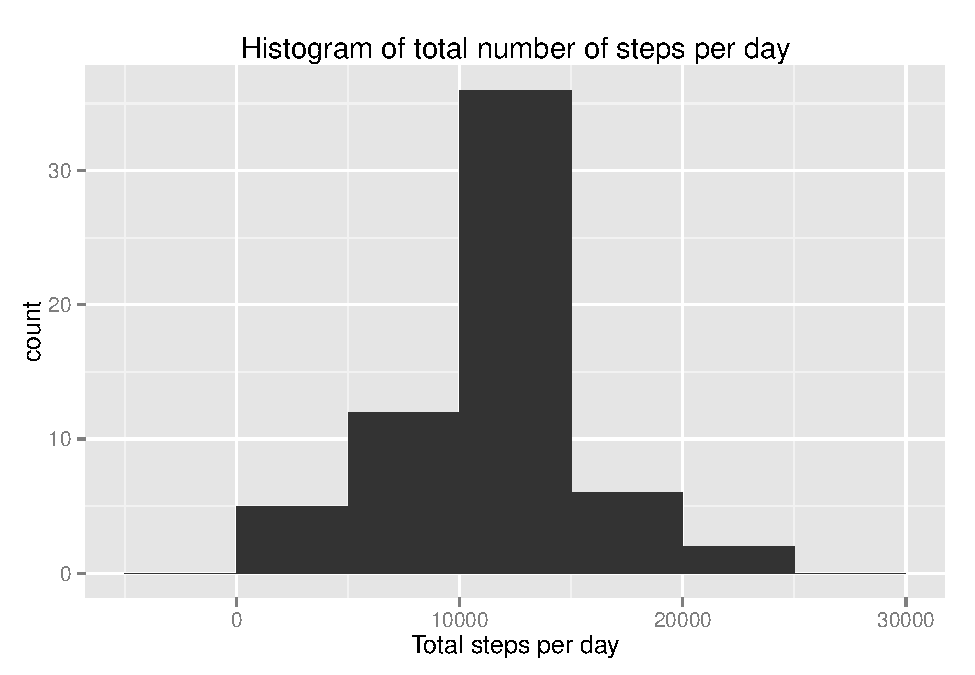
\includegraphics{PA1_template_files/figure-latex/unnamed-chunk-10-1.pdf}

\begin{Shaded}
\begin{Highlighting}[]
\NormalTok{mean <-}\StringTok{ }\KeywordTok{trunc}\NormalTok{(}\KeywordTok{mean}\NormalTok{(Activity.clean.day.sum$total, }\DataTypeTok{na.rm =} \NormalTok{T))}
\NormalTok{median <-}\StringTok{ }\KeywordTok{trunc}\NormalTok{(}\KeywordTok{median}\NormalTok{(Activity.clean.day.sum$total, }\DataTypeTok{na.rm =} \NormalTok{T))}
\end{Highlighting}
\end{Shaded}

Mean and median show slight differences between both datasets.

\section{Are there differences in activity patterns between weekdays and
weekends?}\label{are-there-differences-in-activity-patterns-between-weekdays-and-weekends}

For this part the weekdays() function may be of some help here. Use the
dataset with the filled-in missing values for this part.

Create a new factor variable in the dataset with two levels -
``weekday'' and ``weekend'' indicating whether a given date is a weekday
or weekend day.

Make a panel plot containing a time series plot (i.e.~type = ``l'') of
the 5-minute interval (x-axis) and the average number of steps taken,
averaged across all weekday days or weekend days (y-axis). See the
README file in the GitHub repository to see an example of what this plot
should look like using simulated data.

\begin{Shaded}
\begin{Highlighting}[]
\CommentTok{#New factor variable }
\NormalTok{Activity.clean$wd <-}\StringTok{ }\KeywordTok{ifelse}\NormalTok{(}\KeywordTok{weekdays}\NormalTok{(Activity.clean$date) %in%}\StringTok{ }\KeywordTok{c}\NormalTok{(}\StringTok{"sábado"}\NormalTok{, }\StringTok{"domingo"}\NormalTok{), }\StringTok{"weekend"}\NormalTok{, }\StringTok{"weekday"}\NormalTok{)}
\CommentTok{#Activity.clean$wd <- ifelse((wday(Activity.clean$date) == 1 || wday(Activity.clean$date) == 7),"weekend","weekday")}

\NormalTok{Activity.clean$wd<-}\StringTok{ }\KeywordTok{as.factor}\NormalTok{(Activity.clean$wd)}


\NormalTok{Activity.clean.wd <-}\StringTok{ }\KeywordTok{group_by}\NormalTok{(Activity.clean, interval, wd)}
\NormalTok{Activity.clean.wd.avg <-}\StringTok{ }\KeywordTok{summarise}\NormalTok{(Activity.clean.wd, }\DataTypeTok{avg =} \KeywordTok{mean}\NormalTok{(steps))}



\NormalTok{g <-}\StringTok{ }\KeywordTok{ggplot}\NormalTok{(Activity.clean.wd.avg, }\KeywordTok{aes}\NormalTok{(interval, avg))}
\NormalTok{g +}\StringTok{ }\KeywordTok{geom_line}\NormalTok{() +}\StringTok{ }\KeywordTok{facet_grid}\NormalTok{(wd ~}\StringTok{ }\NormalTok{.) }
\end{Highlighting}
\end{Shaded}

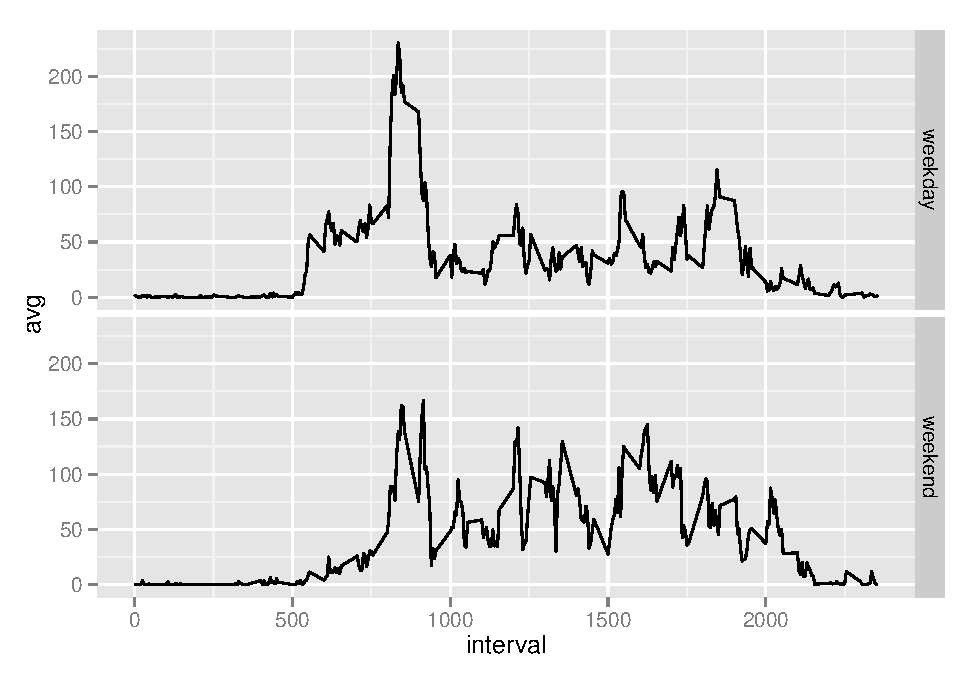
\includegraphics{PA1_template_files/figure-latex/unnamed-chunk-12-1.pdf}

Yes, it seems there are a lot of differences between weekdays and
weekends. People tend to wake up later. During weekdays the activity
peak is at 8:35 am whereas in the weekend the peaks are around 10:00 am
and 4:00 pm

\end{document}
